% Created by tikzDevice version 0.12.3.1 on 2022-03-17 12:11:05
% !TEX encoding = UTF-8 Unicode
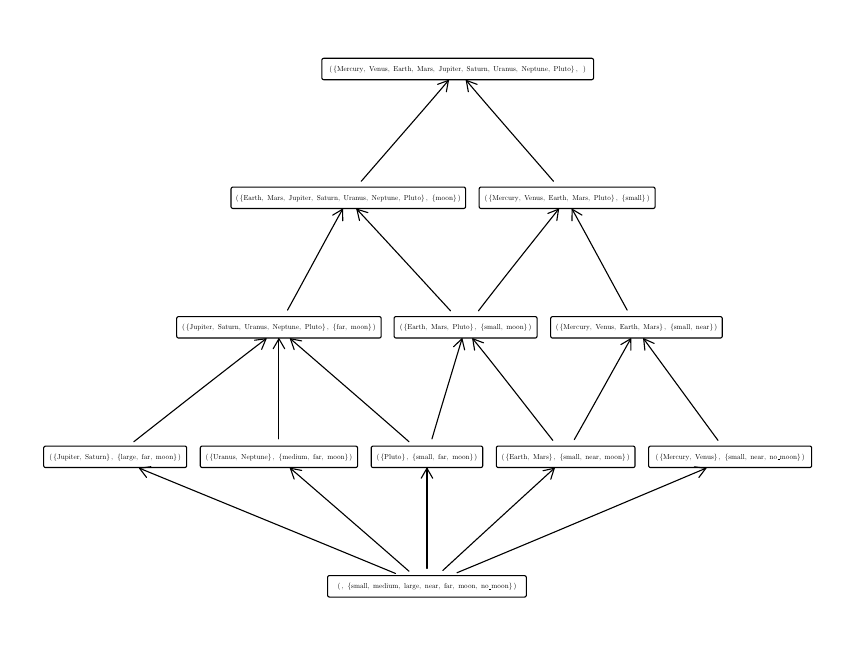
\begin{tikzpicture}[x=1pt,y=1pt]
\definecolor{fillColor}{RGB}{255,255,255}
\path[use as bounding box,fill=fillColor,fill opacity=0.00] (0,0) rectangle (289.08,216.81);
\begin{scope}
\path[clip] (  0.00,  0.00) rectangle (289.08,216.81);
\definecolor{drawColor}{RGB}{0,0,0}

\path[draw=drawColor,line width= 0.4pt,line join=round,line cap=round] (107.07,197.99) --
	(203.71,197.99) --
	(203.68,198.00) --
	(203.81,198.00) --
	(203.93,198.03) --
	(204.04,198.07) --
	(204.15,198.13) --
	(204.25,198.21) --
	(204.33,198.30) --
	(204.40,198.41) --
	(204.45,198.52) --
	(204.48,198.65) --
	(204.49,198.77) --
	(204.49,198.77) --
	(204.49,204.98) --
	(204.49,204.98) --
	(204.48,205.10) --
	(204.45,205.22) --
	(204.40,205.34) --
	(204.33,205.44) --
	(204.25,205.54) --
	(204.15,205.61) --
	(204.04,205.68) --
	(203.93,205.72) --
	(203.81,205.75) --
	(203.71,205.75) --
	(107.07,205.75) --
	(107.17,205.75) --
	(107.04,205.75) --
	(106.92,205.74) --
	(106.80,205.70) --
	(106.69,205.65) --
	(106.58,205.58) --
	(106.49,205.49) --
	(106.42,205.39) --
	(106.36,205.28) --
	(106.32,205.16) --
	(106.30,205.04) --
	(106.30,204.98) --
	(106.30,198.77) --
	(106.30,198.83) --
	(106.30,198.71) --
	(106.32,198.58) --
	(106.36,198.47) --
	(106.42,198.36) --
	(106.49,198.26) --
	(106.58,198.17) --
	(106.69,198.10) --
	(106.80,198.05) --
	(106.92,198.01) --
	(107.04,198.00) --
	cycle;
\end{scope}
\begin{scope}
\path[clip] (106.30,197.99) rectangle (204.49,205.75);
\definecolor{drawColor}{RGB}{0,0,0}

\node[text=drawColor,anchor=base,inner sep=0pt, outer sep=0pt, scale=  0.26] at (155.39,200.99) {$\left(\,\ensuremath{\left\{\mathrm{Mercury},\,\,\mathrm{Venus},\,\,\mathrm{Earth},\,\,\mathrm{Mars},\,\,\mathrm{Jupiter},\,\,\mathrm{Saturn},\,\,\mathrm{Uranus},\,\,\mathrm{Neptune},\,\,\mathrm{Pluto}\right\}},\right.\left.\ensuremath{\varnothing}\,\right)$};
\end{scope}
\begin{scope}
\path[clip] (  0.00,  0.00) rectangle (289.08,216.81);
\definecolor{drawColor}{RGB}{0,0,0}

\path[draw=drawColor,line width= 0.4pt,line join=round,line cap=round] ( 74.26,151.45) --
	(157.46,151.45) --
	(157.43,151.46) --
	(157.55,151.46) --
	(157.68,151.49) --
	(157.79,151.53) --
	(157.90,151.59) --
	(158.00,151.67) --
	(158.08,151.76) --
	(158.15,151.87) --
	(158.20,151.98) --
	(158.22,152.11) --
	(158.23,152.23) --
	(158.23,152.23) --
	(158.23,158.44) --
	(158.23,158.44) --
	(158.22,158.56) --
	(158.20,158.68) --
	(158.15,158.80) --
	(158.08,158.90) --
	(158.00,159.00) --
	(157.90,159.07) --
	(157.79,159.14) --
	(157.68,159.18) --
	(157.55,159.21) --
	(157.46,159.21) --
	( 74.26,159.21) --
	( 74.35,159.21) --
	( 74.23,159.21) --
	( 74.10,159.20) --
	( 73.98,159.16) --
	( 73.87,159.11) --
	( 73.77,159.04) --
	( 73.68,158.95) --
	( 73.60,158.85) --
	( 73.54,158.74) --
	( 73.50,158.62) --
	( 73.48,158.50) --
	( 73.48,158.44) --
	( 73.48,152.23) --
	( 73.48,152.29) --
	( 73.48,152.17) --
	( 73.50,152.04) --
	( 73.54,151.93) --
	( 73.60,151.82) --
	( 73.68,151.72) --
	( 73.77,151.63) --
	( 73.87,151.56) --
	( 73.98,151.50) --
	( 74.10,151.47) --
	( 74.23,151.46) --
	cycle;
\end{scope}
\begin{scope}
\path[clip] ( 73.48,151.45) rectangle (158.23,159.21);
\definecolor{drawColor}{RGB}{0,0,0}

\node[text=drawColor,anchor=base,inner sep=0pt, outer sep=0pt, scale=  0.26] at (115.86,154.45) {$\left(\,\ensuremath{\left\{\mathrm{Earth},\,\,\mathrm{Mars},\,\,\mathrm{Jupiter},\,\,\mathrm{Saturn},\,\,\mathrm{Uranus},\,\,\mathrm{Neptune},\,\,\mathrm{Pluto}\right\}},\right.\left.\ensuremath{\left\{\mathrm{moon}\right\}}\,\right)$};
\end{scope}
\begin{scope}
\path[clip] (  0.00,  0.00) rectangle (289.08,216.81);
\definecolor{drawColor}{RGB}{0,0,0}

\path[draw=drawColor,line width= 0.4pt,line join=round,line cap=round] ( 54.62,104.66) --
	(126.97,104.66) --
	(126.94,104.66) --
	(127.06,104.66) --
	(127.18,104.69) --
	(127.30,104.73) --
	(127.41,104.79) --
	(127.51,104.87) --
	(127.59,104.97) --
	(127.66,105.07) --
	(127.70,105.19) --
	(127.73,105.31) --
	(127.74,105.43) --
	(127.74,105.43) --
	(127.74,111.64) --
	(127.74,111.64) --
	(127.73,111.76) --
	(127.70,111.88) --
	(127.66,112.00) --
	(127.59,112.10) --
	(127.51,112.20) --
	(127.41,112.28) --
	(127.30,112.34) --
	(127.18,112.38) --
	(127.06,112.41) --
	(126.97,112.41) --
	( 54.62,112.41) --
	( 54.71,112.41) --
	( 54.59,112.41) --
	( 54.46,112.40) --
	( 54.34,112.36) --
	( 54.23,112.31) --
	( 54.13,112.24) --
	( 54.04,112.15) --
	( 53.96,112.05) --
	( 53.91,111.94) --
	( 53.87,111.82) --
	( 53.85,111.70) --
	( 53.84,111.64) --
	( 53.84,105.43) --
	( 53.85,105.49) --
	( 53.85,105.37) --
	( 53.87,105.25) --
	( 53.91,105.13) --
	( 53.96,105.02) --
	( 54.04,104.92) --
	( 54.13,104.83) --
	( 54.23,104.76) --
	( 54.34,104.71) --
	( 54.46,104.67) --
	( 54.59,104.66) --
	cycle;
\end{scope}
\begin{scope}
\path[clip] ( 53.84,104.66) rectangle (127.74,112.41);
\definecolor{drawColor}{RGB}{0,0,0}

\node[text=drawColor,anchor=base,inner sep=0pt, outer sep=0pt, scale=  0.26] at ( 90.79,107.65) {$\left(\,\ensuremath{\left\{\mathrm{Jupiter},\,\,\mathrm{Saturn},\,\,\mathrm{Uranus},\,\,\mathrm{Neptune},\,\,\mathrm{Pluto}\right\}},\right.\left.\ensuremath{\left\{\mathrm{far},\,\,\mathrm{moon}\right\}}\,\right)$};
\end{scope}
\begin{scope}
\path[clip] (  0.00,  0.00) rectangle (289.08,216.81);
\definecolor{drawColor}{RGB}{0,0,0}

\path[draw=drawColor,line width= 0.4pt,line join=round,line cap=round] (  6.56, 57.86) --
	( 56.69, 57.86) --
	( 56.65, 57.86) --
	( 56.78, 57.86) --
	( 56.90, 57.89) --
	( 57.02, 57.93) --
	( 57.13, 57.99) --
	( 57.22, 58.07) --
	( 57.31, 58.17) --
	( 57.37, 58.27) --
	( 57.42, 58.39) --
	( 57.45, 58.51) --
	( 57.46, 58.63) --
	( 57.46, 58.63) --
	( 57.46, 64.84) --
	( 57.46, 64.84) --
	( 57.45, 64.96) --
	( 57.42, 65.08) --
	( 57.37, 65.20) --
	( 57.31, 65.30) --
	( 57.22, 65.40) --
	( 57.13, 65.48) --
	( 57.02, 65.54) --
	( 56.90, 65.58) --
	( 56.78, 65.61) --
	( 56.69, 65.61) --
	(  6.56, 65.61) --
	(  6.65, 65.61) --
	(  6.53, 65.61) --
	(  6.40, 65.60) --
	(  6.28, 65.56) --
	(  6.17, 65.51) --
	(  6.07, 65.44) --
	(  5.98, 65.35) --
	(  5.90, 65.25) --
	(  5.84, 65.14) --
	(  5.80, 65.02) --
	(  5.78, 64.90) --
	(  5.78, 64.84) --
	(  5.78, 58.63) --
	(  5.78, 58.70) --
	(  5.78, 58.57) --
	(  5.80, 58.45) --
	(  5.84, 58.33) --
	(  5.90, 58.22) --
	(  5.98, 58.12) --
	(  6.07, 58.03) --
	(  6.17, 57.96) --
	(  6.28, 57.91) --
	(  6.40, 57.87) --
	(  6.53, 57.86) --
	cycle;
\end{scope}
\begin{scope}
\path[clip] (  5.78, 57.86) rectangle ( 57.46, 65.61);
\definecolor{drawColor}{RGB}{0,0,0}

\node[text=drawColor,anchor=base,inner sep=0pt, outer sep=0pt, scale=  0.26] at ( 31.62, 60.85) {$\left(\,\ensuremath{\left\{\mathrm{Jupiter},\,\,\mathrm{Saturn}\right\}},\right.\left.\ensuremath{\left\{\mathrm{large},\,\,\mathrm{far},\,\,\mathrm{moon}\right\}}\,\right)$};
\end{scope}
\begin{scope}
\path[clip] (  0.00,  0.00) rectangle (289.08,216.81);
\definecolor{drawColor}{RGB}{0,0,0}

\path[draw=drawColor,line width= 0.4pt,line join=round,line cap=round] ( 63.15, 57.86) --
	(118.44, 57.86) --
	(118.41, 57.86) --
	(118.54, 57.86) --
	(118.66, 57.89) --
	(118.77, 57.93) --
	(118.88, 57.99) --
	(118.98, 58.07) --
	(119.06, 58.17) --
	(119.13, 58.27) --
	(119.18, 58.39) --
	(119.21, 58.51) --
	(119.22, 58.63) --
	(119.22, 58.63) --
	(119.22, 64.84) --
	(119.22, 64.84) --
	(119.21, 64.96) --
	(119.18, 65.08) --
	(119.13, 65.20) --
	(119.06, 65.30) --
	(118.98, 65.40) --
	(118.88, 65.48) --
	(118.77, 65.54) --
	(118.66, 65.58) --
	(118.54, 65.61) --
	(118.44, 65.61) --
	( 63.15, 65.61) --
	( 63.24, 65.61) --
	( 63.11, 65.61) --
	( 62.99, 65.60) --
	( 62.87, 65.56) --
	( 62.76, 65.51) --
	( 62.66, 65.44) --
	( 62.57, 65.35) --
	( 62.49, 65.25) --
	( 62.43, 65.14) --
	( 62.39, 65.02) --
	( 62.37, 64.90) --
	( 62.37, 64.84) --
	( 62.37, 58.63) --
	( 62.37, 58.70) --
	( 62.37, 58.57) --
	( 62.39, 58.45) --
	( 62.43, 58.33) --
	( 62.49, 58.22) --
	( 62.57, 58.12) --
	( 62.66, 58.03) --
	( 62.76, 57.96) --
	( 62.87, 57.91) --
	( 62.99, 57.87) --
	( 63.11, 57.86) --
	cycle;
\end{scope}
\begin{scope}
\path[clip] ( 62.37, 57.86) rectangle (119.22, 65.61);
\definecolor{drawColor}{RGB}{0,0,0}

\node[text=drawColor,anchor=base,inner sep=0pt, outer sep=0pt, scale=  0.26] at ( 90.79, 60.85) {$\left(\,\ensuremath{\left\{\mathrm{Uranus},\,\,\mathrm{Neptune}\right\}},\right.\left.\ensuremath{\left\{\mathrm{medium},\,\,\mathrm{far},\,\,\mathrm{moon}\right\}}\,\right)$};
\end{scope}
\begin{scope}
\path[clip] (  0.00,  0.00) rectangle (289.08,216.81);
\definecolor{drawColor}{RGB}{0,0,0}

\path[draw=drawColor,line width= 0.4pt,line join=round,line cap=round] (163.92,151.45) --
	(225.93,151.45) --
	(225.90,151.46) --
	(226.03,151.46) --
	(226.15,151.49) --
	(226.27,151.53) --
	(226.37,151.59) --
	(226.47,151.67) --
	(226.55,151.76) --
	(226.62,151.87) --
	(226.67,151.98) --
	(226.70,152.11) --
	(226.71,152.23) --
	(226.71,152.23) --
	(226.71,158.44) --
	(226.71,158.44) --
	(226.70,158.56) --
	(226.67,158.68) --
	(226.62,158.80) --
	(226.55,158.90) --
	(226.47,159.00) --
	(226.37,159.07) --
	(226.27,159.14) --
	(226.15,159.18) --
	(226.03,159.21) --
	(225.93,159.21) --
	(163.92,159.21) --
	(164.01,159.21) --
	(163.89,159.21) --
	(163.76,159.20) --
	(163.65,159.16) --
	(163.53,159.11) --
	(163.43,159.04) --
	(163.34,158.95) --
	(163.26,158.85) --
	(163.21,158.74) --
	(163.17,158.62) --
	(163.15,158.50) --
	(163.14,158.44) --
	(163.14,152.23) --
	(163.15,152.29) --
	(163.15,152.17) --
	(163.17,152.04) --
	(163.21,151.93) --
	(163.26,151.82) --
	(163.34,151.72) --
	(163.43,151.63) --
	(163.53,151.56) --
	(163.65,151.50) --
	(163.76,151.47) --
	(163.89,151.46) --
	cycle;
\end{scope}
\begin{scope}
\path[clip] (163.14,151.45) rectangle (226.71,159.21);
\definecolor{drawColor}{RGB}{0,0,0}

\node[text=drawColor,anchor=base,inner sep=0pt, outer sep=0pt, scale=  0.26] at (194.93,154.45) {$\left(\,\ensuremath{\left\{\mathrm{Mercury},\,\,\mathrm{Venus},\,\,\mathrm{Earth},\,\,\mathrm{Mars},\,\,\mathrm{Pluto}\right\}},\right.\left.\ensuremath{\left\{\mathrm{small}\right\}}\,\right)$};
\end{scope}
\begin{scope}
\path[clip] (  0.00,  0.00) rectangle (289.08,216.81);
\definecolor{drawColor}{RGB}{0,0,0}

\path[draw=drawColor,line width= 0.4pt,line join=round,line cap=round] (133.17,104.66) --
	(183.30,104.66) --
	(183.27,104.66) --
	(183.39,104.66) --
	(183.51,104.69) --
	(183.63,104.73) --
	(183.74,104.79) --
	(183.84,104.87) --
	(183.92,104.97) --
	(183.99,105.07) --
	(184.03,105.19) --
	(184.06,105.31) --
	(184.07,105.43) --
	(184.07,105.43) --
	(184.07,111.64) --
	(184.07,111.64) --
	(184.06,111.76) --
	(184.03,111.88) --
	(183.99,112.00) --
	(183.92,112.10) --
	(183.84,112.20) --
	(183.74,112.28) --
	(183.63,112.34) --
	(183.51,112.38) --
	(183.39,112.41) --
	(183.30,112.41) --
	(133.17,112.41) --
	(133.26,112.41) --
	(133.14,112.41) --
	(133.02,112.40) --
	(132.90,112.36) --
	(132.78,112.31) --
	(132.68,112.24) --
	(132.59,112.15) --
	(132.52,112.05) --
	(132.46,111.94) --
	(132.42,111.82) --
	(132.40,111.70) --
	(132.40,111.64) --
	(132.40,105.43) --
	(132.40,105.49) --
	(132.40,105.37) --
	(132.42,105.25) --
	(132.46,105.13) --
	(132.52,105.02) --
	(132.59,104.92) --
	(132.68,104.83) --
	(132.78,104.76) --
	(132.90,104.71) --
	(133.02,104.67) --
	(133.14,104.66) --
	cycle;
\end{scope}
\begin{scope}
\path[clip] (132.40,104.66) rectangle (184.07,112.41);
\definecolor{drawColor}{RGB}{0,0,0}

\node[text=drawColor,anchor=base,inner sep=0pt, outer sep=0pt, scale=  0.26] at (158.23,107.65) {$\left(\,\ensuremath{\left\{\mathrm{Earth},\,\,\mathrm{Mars},\,\,\mathrm{Pluto}\right\}},\right.\left.\ensuremath{\left\{\mathrm{small},\,\,\mathrm{moon}\right\}}\,\right)$};
\end{scope}
\begin{scope}
\path[clip] (  0.00,  0.00) rectangle (289.08,216.81);
\definecolor{drawColor}{RGB}{0,0,0}

\path[draw=drawColor,line width= 0.4pt,line join=round,line cap=round] (124.90, 57.86) --
	(163.66, 57.86) --
	(163.63, 57.86) --
	(163.75, 57.86) --
	(163.88, 57.89) --
	(163.99, 57.93) --
	(164.10, 57.99) --
	(164.20, 58.07) --
	(164.28, 58.17) --
	(164.35, 58.27) --
	(164.40, 58.39) --
	(164.43, 58.51) --
	(164.44, 58.63) --
	(164.44, 58.63) --
	(164.44, 64.84) --
	(164.44, 64.84) --
	(164.43, 64.96) --
	(164.40, 65.08) --
	(164.35, 65.20) --
	(164.28, 65.30) --
	(164.20, 65.40) --
	(164.10, 65.48) --
	(163.99, 65.54) --
	(163.88, 65.58) --
	(163.75, 65.61) --
	(163.66, 65.61) --
	(124.90, 65.61) --
	(125.00, 65.61) --
	(124.87, 65.61) --
	(124.75, 65.60) --
	(124.63, 65.56) --
	(124.51, 65.51) --
	(124.41, 65.44) --
	(124.32, 65.35) --
	(124.25, 65.25) --
	(124.19, 65.14) --
	(124.15, 65.02) --
	(124.13, 64.90) --
	(124.13, 64.84) --
	(124.13, 58.63) --
	(124.13, 58.70) --
	(124.13, 58.57) --
	(124.15, 58.45) --
	(124.19, 58.33) --
	(124.25, 58.22) --
	(124.32, 58.12) --
	(124.41, 58.03) --
	(124.51, 57.96) --
	(124.63, 57.91) --
	(124.75, 57.87) --
	(124.87, 57.86) --
	cycle;
\end{scope}
\begin{scope}
\path[clip] (124.13, 57.86) rectangle (164.44, 65.61);
\definecolor{drawColor}{RGB}{0,0,0}

\node[text=drawColor,anchor=base,inner sep=0pt, outer sep=0pt, scale=  0.26] at (144.28, 60.86) {$\left(\,\ensuremath{\left\{\mathrm{Pluto}\right\}},\right.\left.\ensuremath{\left\{\mathrm{small},\,\,\mathrm{far},\,\,\mathrm{moon}\right\}}\,\right)$};
\end{scope}
\begin{scope}
\path[clip] (  0.00,  0.00) rectangle (289.08,216.81);
\definecolor{drawColor}{RGB}{0,0,0}

\path[draw=drawColor,line width= 0.4pt,line join=round,line cap=round] (189.76,104.66) --
	(250.22,104.66) --
	(250.19,104.66) --
	(250.32,104.66) --
	(250.44,104.69) --
	(250.56,104.73) --
	(250.66,104.79) --
	(250.76,104.87) --
	(250.84,104.97) --
	(250.91,105.07) --
	(250.96,105.19) --
	(250.99,105.31) --
	(251.00,105.43) --
	(251.00,105.43) --
	(251.00,111.64) --
	(251.00,111.64) --
	(250.99,111.76) --
	(250.96,111.88) --
	(250.91,112.00) --
	(250.84,112.10) --
	(250.76,112.20) --
	(250.66,112.28) --
	(250.56,112.34) --
	(250.44,112.38) --
	(250.32,112.41) --
	(250.22,112.41) --
	(189.76,112.41) --
	(189.85,112.41) --
	(189.73,112.41) --
	(189.60,112.40) --
	(189.48,112.36) --
	(189.37,112.31) --
	(189.27,112.24) --
	(189.18,112.15) --
	(189.10,112.05) --
	(189.05,111.94) --
	(189.01,111.82) --
	(188.99,111.70) --
	(188.98,111.64) --
	(188.98,105.43) --
	(188.99,105.49) --
	(188.99,105.37) --
	(189.01,105.25) --
	(189.05,105.13) --
	(189.10,105.02) --
	(189.18,104.92) --
	(189.27,104.83) --
	(189.37,104.76) --
	(189.48,104.71) --
	(189.60,104.67) --
	(189.73,104.66) --
	cycle;
\end{scope}
\begin{scope}
\path[clip] (188.98,104.66) rectangle (251.00,112.41);
\definecolor{drawColor}{RGB}{0,0,0}

\node[text=drawColor,anchor=base,inner sep=0pt, outer sep=0pt, scale=  0.26] at (219.99,107.65) {$\left(\,\ensuremath{\left\{\mathrm{Mercury},\,\,\mathrm{Venus},\,\,\mathrm{Earth},\,\,\mathrm{Mars}\right\}},\right.\left.\ensuremath{\left\{\mathrm{small},\,\,\mathrm{near}\right\}}\,\right)$};
\end{scope}
\begin{scope}
\path[clip] (  0.00,  0.00) rectangle (289.08,216.81);
\definecolor{drawColor}{RGB}{0,0,0}

\path[draw=drawColor,line width= 0.4pt,line join=round,line cap=round] (225.16, 57.86) --
	(282.52, 57.86) --
	(282.49, 57.86) --
	(282.62, 57.86) --
	(282.74, 57.89) --
	(282.86, 57.93) --
	(282.96, 57.99) --
	(283.06, 58.07) --
	(283.14, 58.17) --
	(283.21, 58.27) --
	(283.26, 58.39) --
	(283.29, 58.51) --
	(283.30, 58.63) --
	(283.30, 58.63) --
	(283.30, 64.84) --
	(283.30, 64.84) --
	(283.29, 64.96) --
	(283.26, 65.08) --
	(283.21, 65.20) --
	(283.14, 65.30) --
	(283.06, 65.40) --
	(282.96, 65.48) --
	(282.86, 65.54) --
	(282.74, 65.58) --
	(282.62, 65.61) --
	(282.52, 65.61) --
	(225.16, 65.61) --
	(225.25, 65.61) --
	(225.13, 65.61) --
	(225.00, 65.60) --
	(224.88, 65.56) --
	(224.77, 65.51) --
	(224.67, 65.44) --
	(224.58, 65.35) --
	(224.50, 65.25) --
	(224.45, 65.14) --
	(224.41, 65.02) --
	(224.39, 64.90) --
	(224.38, 64.84) --
	(224.38, 58.63) --
	(224.39, 58.70) --
	(224.39, 58.57) --
	(224.41, 58.45) --
	(224.45, 58.33) --
	(224.50, 58.22) --
	(224.58, 58.12) --
	(224.67, 58.03) --
	(224.77, 57.96) --
	(224.88, 57.91) --
	(225.00, 57.87) --
	(225.13, 57.86) --
	cycle;
\end{scope}
\begin{scope}
\path[clip] (224.38, 57.86) rectangle (283.30, 65.61);
\definecolor{drawColor}{RGB}{0,0,0}

\node[text=drawColor,anchor=base,inner sep=0pt, outer sep=0pt, scale=  0.26] at (253.84, 60.85) {$\left(\,\ensuremath{\left\{\mathrm{Mercury},\,\,\mathrm{Venus}\right\}},\right.\left.\ensuremath{\left\{\mathrm{small},\,\,\mathrm{near},\,\,\mathrm{no\_moon}\right\}}\,\right)$};
\end{scope}
\begin{scope}
\path[clip] (  0.00,  0.00) rectangle (289.08,216.81);
\definecolor{drawColor}{RGB}{0,0,0}

\path[draw=drawColor,line width= 0.4pt,line join=round,line cap=round] (170.12, 57.86) --
	(218.70, 57.86) --
	(218.67, 57.86) --
	(218.79, 57.86) --
	(218.91, 57.89) --
	(219.03, 57.93) --
	(219.14, 57.99) --
	(219.24, 58.07) --
	(219.32, 58.17) --
	(219.39, 58.27) --
	(219.43, 58.39) --
	(219.46, 58.51) --
	(219.47, 58.63) --
	(219.47, 58.63) --
	(219.47, 64.84) --
	(219.47, 64.84) --
	(219.46, 64.96) --
	(219.43, 65.08) --
	(219.39, 65.20) --
	(219.32, 65.30) --
	(219.24, 65.40) --
	(219.14, 65.48) --
	(219.03, 65.54) --
	(218.91, 65.58) --
	(218.79, 65.61) --
	(218.70, 65.61) --
	(170.12, 65.61) --
	(170.22, 65.61) --
	(170.09, 65.61) --
	(169.97, 65.60) --
	(169.85, 65.56) --
	(169.73, 65.51) --
	(169.63, 65.44) --
	(169.54, 65.35) --
	(169.47, 65.25) --
	(169.41, 65.14) --
	(169.37, 65.02) --
	(169.35, 64.90) --
	(169.35, 64.84) --
	(169.35, 58.63) --
	(169.35, 58.70) --
	(169.35, 58.57) --
	(169.37, 58.45) --
	(169.41, 58.33) --
	(169.47, 58.22) --
	(169.54, 58.12) --
	(169.63, 58.03) --
	(169.73, 57.96) --
	(169.85, 57.91) --
	(169.97, 57.87) --
	(170.09, 57.86) --
	cycle;
\end{scope}
\begin{scope}
\path[clip] (169.35, 57.86) rectangle (219.47, 65.61);
\definecolor{drawColor}{RGB}{0,0,0}

\node[text=drawColor,anchor=base,inner sep=0pt, outer sep=0pt, scale=  0.26] at (194.41, 60.85) {$\left(\,\ensuremath{\left\{\mathrm{Earth},\,\,\mathrm{Mars}\right\}},\right.\left.\ensuremath{\left\{\mathrm{small},\,\,\mathrm{near},\,\,\mathrm{moon}\right\}}\,\right)$};
\end{scope}
\begin{scope}
\path[clip] (  0.00,  0.00) rectangle (289.08,216.81);
\definecolor{drawColor}{RGB}{0,0,0}

\path[draw=drawColor,line width= 0.4pt,line join=round,line cap=round] (109.14, 11.06) --
	(179.42, 11.06) --
	(179.39, 11.06) --
	(179.52, 11.06) --
	(179.64, 11.09) --
	(179.76, 11.13) --
	(179.86, 11.20) --
	(179.96, 11.27) --
	(180.04, 11.37) --
	(180.11, 11.47) --
	(180.16, 11.59) --
	(180.19, 11.71) --
	(180.20, 11.83) --
	(180.20, 11.83) --
	(180.20, 18.04) --
	(180.20, 18.04) --
	(180.19, 18.16) --
	(180.16, 18.29) --
	(180.11, 18.40) --
	(180.04, 18.51) --
	(179.96, 18.60) --
	(179.86, 18.68) --
	(179.76, 18.74) --
	(179.64, 18.78) --
	(179.52, 18.81) --
	(179.42, 18.82) --
	(109.14, 18.82) --
	(109.23, 18.81) --
	(109.11, 18.81) --
	(108.99, 18.80) --
	(108.87, 18.76) --
	(108.75, 18.71) --
	(108.65, 18.64) --
	(108.56, 18.55) --
	(108.48, 18.45) --
	(108.43, 18.34) --
	(108.39, 18.23) --
	(108.37, 18.10) --
	(108.36, 18.04) --
	(108.36, 11.83) --
	(108.37, 11.90) --
	(108.37, 11.77) --
	(108.39, 11.65) --
	(108.43, 11.53) --
	(108.48, 11.42) --
	(108.56, 11.32) --
	(108.65, 11.23) --
	(108.75, 11.16) --
	(108.87, 11.11) --
	(108.99, 11.07) --
	(109.11, 11.06) --
	cycle;
\end{scope}
\begin{scope}
\path[clip] (108.36, 11.06) rectangle (180.20, 18.82);
\definecolor{drawColor}{RGB}{0,0,0}

\node[text=drawColor,anchor=base,inner sep=0pt, outer sep=0pt, scale=  0.26] at (144.28, 14.05) {$\left(\,\ensuremath{\varnothing},\right.\left.\ensuremath{\left\{\mathrm{small},\,\,\mathrm{medium},\,\,\mathrm{large},\,\,\mathrm{near},\,\,\mathrm{far},\,\,\mathrm{moon},\,\,\mathrm{no\_moon}\right\}}\,\right)$};
\end{scope}
\begin{scope}
\path[clip] (  0.00,  0.00) rectangle (289.08,216.81);
\definecolor{drawColor}{RGB}{0,0,0}

\path[draw=drawColor,line width= 0.4pt,line join=round,line cap=round] (152.03,197.74) --
	(149.74,195.03) --
	(146.97,191.79) --
	(143.82,188.13) --
	(140.42,184.20) --
	(136.85,180.09) --
	(133.24,175.94) --
	(129.70,171.86) --
	(126.32,167.98) --
	(123.22,164.41) --
	(120.51,161.28);

\path[draw=drawColor,line width= 0.4pt,line join=round,line cap=round] (151.29,193.64) --
	(152.03,197.74) --
	(148.12,196.33);

\path[draw=drawColor,line width= 0.4pt,line join=round,line cap=round] (158.49,197.74) --
	(160.79,195.03) --
	(163.56,191.79) --
	(166.70,188.13) --
	(170.11,184.20) --
	(173.67,180.09) --
	(177.28,175.94) --
	(180.83,171.86) --
	(184.21,167.98) --
	(187.31,164.41) --
	(190.02,161.28);

\path[draw=drawColor,line width= 0.4pt,line join=round,line cap=round] (162.41,196.33) --
	(158.49,197.74) --
	(159.23,193.64);

\path[draw=drawColor,line width= 0.4pt,line join=round,line cap=round] (113.79,151.20) --
	(112.31,148.56) --
	(110.56,145.37) --
	(108.58,141.76) --
	(106.45,137.84) --
	(104.23,133.74) --
	(101.98,129.58) --
	( 99.75,125.48) --
	( 97.63,121.56) --
	( 95.65,117.94) --
	( 93.89,114.74);

\path[draw=drawColor,line width= 0.4pt,line join=round,line cap=round] (113.85,147.03) --
	(113.79,151.20) --
	(110.21,149.07);

\path[draw=drawColor,line width= 0.4pt,line join=round,line cap=round] (118.96,151.20) --
	(121.49,148.48) --
	(124.51,145.22) --
	(127.91,141.54) --
	(131.58,137.56) --
	(135.40,133.42) --
	(139.26,129.23) --
	(143.04,125.12) --
	(146.63,121.20) --
	(149.93,117.62) --
	(152.81,114.48);

\path[draw=drawColor,line width= 0.4pt,line join=round,line cap=round] (122.94,149.98) --
	(118.96,151.20) --
	(119.89,147.14);

\path[draw=drawColor,line width= 0.4pt,line join=round,line cap=round] ( 86.14,104.40) --
	( 82.56,101.67) --
	( 78.27, 98.37) --
	( 73.44, 94.63) --
	( 68.24, 90.58) --
	( 62.82, 86.36) --
	( 57.36, 82.10) --
	( 52.02, 77.91) --
	( 46.96, 73.94) --
	( 42.34, 70.32) --
	( 38.34, 67.17);

\path[draw=drawColor,line width= 0.4pt,line join=round,line cap=round] ( 84.54,100.56) --
	( 86.14,104.40) --
	( 82.01,103.87);

\path[draw=drawColor,line width= 0.4pt,line join=round,line cap=round] ( 90.79,104.40) --
	( 90.79,101.76) --
	( 90.79, 98.60) --
	( 90.79, 95.01) --
	( 90.79, 91.13) --
	( 90.79, 87.07) --
	( 90.79, 82.95) --
	( 90.79, 78.89) --
	( 90.79, 74.99) --
	( 90.79, 71.39) --
	( 90.79, 68.20);

\path[draw=drawColor,line width= 0.4pt,line join=round,line cap=round] ( 92.88,100.79) --
	( 90.79,104.40) --
	( 88.71,100.79);

\path[draw=drawColor,line width= 0.4pt,line join=round,line cap=round] ( 94.93,104.40) --
	( 98.10,101.67) --
	(101.92, 98.37) --
	(106.24, 94.63) --
	(110.92, 90.58) --
	(115.79, 86.36) --
	(120.71, 82.10) --
	(125.53, 77.91) --
	(130.09, 73.94) --
	(134.23, 70.32) --
	(137.82, 67.17);

\path[draw=drawColor,line width= 0.4pt,line join=round,line cap=round] ( 99.02,103.62) --
	( 94.93,104.40) --
	( 96.30,100.47);

\path[draw=drawColor,line width= 0.4pt,line join=round,line cap=round] ( 40.41, 57.60) --
	( 47.29, 54.78) --
	( 55.61, 51.36) --
	( 65.03, 47.50) --
	( 75.20, 43.33) --
	( 85.79, 38.98) --
	( 96.44, 34.61) --
	(106.83, 30.34) --
	(116.59, 26.32) --
	(125.40, 22.69) --
	(132.91, 19.59);

\path[draw=drawColor,line width= 0.4pt,line join=round,line cap=round] ( 44.53, 58.16) --
	( 40.41, 57.60) --
	( 42.95, 54.30);

\path[draw=drawColor,line width= 0.4pt,line join=round,line cap=round] ( 94.93, 57.60) --
	( 98.10, 54.87) --
	(101.92, 51.57) --
	(106.24, 47.83) --
	(110.92, 43.79) --
	(115.79, 39.56) --
	(120.71, 35.30) --
	(125.53, 31.11) --
	(130.09, 27.14) --
	(134.23, 23.52) --
	(137.82, 20.37);

\path[draw=drawColor,line width= 0.4pt,line join=round,line cap=round] ( 99.02, 56.82) --
	( 94.93, 57.60) --
	( 96.30, 53.67);

\path[draw=drawColor,line width= 0.4pt,line join=round,line cap=round] (191.83,151.20) --
	(189.71,148.55) --
	(187.15,145.34) --
	(184.26,141.70) --
	(181.12,137.75) --
	(177.84,133.61) --
	(174.52,129.42) --
	(171.27,125.28) --
	(168.18,121.33) --
	(165.35,117.69) --
	(162.89,114.48);

\path[draw=drawColor,line width= 0.4pt,line join=round,line cap=round] (191.20,147.08) --
	(191.83,151.20) --
	(187.95,149.68);

\path[draw=drawColor,line width= 0.4pt,line join=round,line cap=round] (196.74,151.20) --
	(198.21,148.56) --
	(199.97,145.37) --
	(201.95,141.76) --
	(204.07,137.84) --
	(206.30,133.74) --
	(208.55,129.58) --
	(210.77,125.48) --
	(212.90,121.56) --
	(214.88,117.94) --
	(216.63,114.74);

\path[draw=drawColor,line width= 0.4pt,line join=round,line cap=round] (200.31,149.07) --
	(196.74,151.20) --
	(196.68,147.03);

\path[draw=drawColor,line width= 0.4pt,line join=round,line cap=round] (156.94,104.40) --
	(156.15,101.76) --
	(155.19, 98.60) --
	(154.11, 95.01) --
	(152.94, 91.13) --
	(151.71, 87.07) --
	(150.47, 82.95) --
	(149.25, 78.89) --
	(148.09, 74.99) --
	(147.02, 71.39) --
	(146.09, 68.20);

\path[draw=drawColor,line width= 0.4pt,line join=round,line cap=round] (157.90,100.35) --
	(156.94,104.40) --
	(153.91,101.54);

\path[draw=drawColor,line width= 0.4pt,line join=round,line cap=round] (160.82,104.40) --
	(162.99,101.75) --
	(165.57, 98.54) --
	(168.45, 94.90) --
	(171.56, 90.95) --
	(174.80, 86.82) --
	(178.08, 82.62) --
	(181.31, 78.48) --
	(184.39, 74.53) --
	(187.24, 70.89) --
	(189.76, 67.68);

\path[draw=drawColor,line width= 0.4pt,line join=round,line cap=round] (164.71,102.93) --
	(160.82,104.40) --
	(161.50,100.29);

\path[draw=drawColor,line width= 0.4pt,line join=round,line cap=round] (144.28, 57.60) --
	(144.28, 54.97) --
	(144.28, 51.80) --
	(144.28, 48.22) --
	(144.28, 44.34) --
	(144.28, 40.28) --
	(144.28, 36.15) --
	(144.28, 32.09) --
	(144.28, 28.19) --
	(144.28, 24.59) --
	(144.28, 21.40);

\path[draw=drawColor,line width= 0.4pt,line join=round,line cap=round] (146.36, 53.99) --
	(144.28, 57.60) --
	(142.20, 53.99);

\path[draw=drawColor,line width= 0.4pt,line join=round,line cap=round] (222.58,104.40) --
	(224.51,101.75) --
	(226.86, 98.54) --
	(229.52, 94.90) --
	(232.41, 90.95) --
	(235.43, 86.82) --
	(238.50, 82.62) --
	(241.53, 78.48) --
	(244.42, 74.53) --
	(247.09, 70.89) --
	(249.45, 67.68);

\path[draw=drawColor,line width= 0.4pt,line join=round,line cap=round] (226.38,102.72) --
	(222.58,104.40) --
	(223.03,100.26);

\path[draw=drawColor,line width= 0.4pt,line join=round,line cap=round] (217.92,104.40) --
	(216.43,101.75) --
	(214.64, 98.55) --
	(212.60, 94.91) --
	(210.40, 90.97) --
	(208.11, 86.85) --
	(205.78, 82.67) --
	(203.48, 78.57) --
	(201.30, 74.66) --
	(199.28, 71.08) --
	(197.51, 67.94);

\path[draw=drawColor,line width= 0.4pt,line join=round,line cap=round] (217.97,100.23) --
	(217.92,104.40) --
	(214.34,102.28);

\path[draw=drawColor,line width= 0.4pt,line join=round,line cap=round] (245.06, 57.60) --
	(238.36, 54.78) --
	(230.27, 51.36) --
	(221.12, 47.51) --
	(211.25, 43.34) --
	(200.97, 39.02) --
	(190.62, 34.66) --
	(180.53, 30.43) --
	(171.03, 26.46) --
	(162.46, 22.88) --
	(155.13, 19.85);

\path[draw=drawColor,line width= 0.4pt,line join=round,line cap=round] (242.54, 54.28) --
	(245.06, 57.60) --
	(240.93, 58.12);

\path[draw=drawColor,line width= 0.4pt,line join=round,line cap=round] (190.28, 57.60) --
	(187.29, 54.87) --
	(183.70, 51.59) --
	(179.65, 47.89) --
	(175.27, 43.88) --
	(170.70, 39.69) --
	(166.09, 35.46) --
	(161.57, 31.32) --
	(157.28, 27.37) --
	(153.37, 23.77) --
	(149.97, 20.63);

\path[draw=drawColor,line width= 0.4pt,line join=round,line cap=round] (189.02, 53.63) --
	(190.28, 57.60) --
	(186.21, 56.71);
\end{scope}
\end{tikzpicture}